%Review of timbral control research.
%	Timbre Definition
%	Timbre Spaces (MDS and shit)
%	Audio Features
%	Perceptual Control of Synthesis

\chapter{Review of Timbral Literature}
\label{chap:Timbre}

\section{Introduction}
\label{sec:Timbre-Introduction}
	This chapter will review the existing body of timbral research, defining timbre and discussing how it is
	investigated. There are three properties that describe the perception of sound, these being loudness, pitch and
	timbre.  Loudness describes the perceived intensity of a sound and pitch its perceived frequency. Timbre then
	describes any other properties of the sound, besides loudness and pitch, which allow it to be distinguished from
	other sounds \citep{mathews1999introduction}. The relationship between perceived loudness and the statistical
	properties of a signal is nonlinear. Despite this, loudness can be expressed using a single dimension: from quiet
	to loud. For a given listener an audio stimulus can only be perceived as quieter than, equally loud as or louder
	than another stimuli. The description of pitch is more complicated as not all stimuli have a single perceived
	pitch. Some stimuli contain several perceived pitches (such as a chord played on a piano) while others do not have
	a pitch (such as white noise). Once the pitches present in a stimuli have been determined they can be compared
	using a single dimension: from low to high pitch. The perception of timbre is more complex still, consisting of
	multiple dimensions \citep{rossing2002the}. There is a large body of research concerning the analysis of timbre,
	identifying these dimensions and their relationships with the acoustic features of a sound.

	A simple interpretation of timbre is that of instrument identification. One can identify the instrument which
	produced a sound from the sound's timbre. This concept can be used to describe the timbre of other sounds, a sound
	could be described as `cello-like' or `flute-like'. More broadly, the class of instrument (e.g. string or woodwind)
	could be used to describe the timbre of a sound. While these terms are useful for discussing the instrumentation of
	pieces of music they can not be applied generally to a wide range of timbres. It is not very useful to describe the
	timbre of a xylophone as being `not flute-like'. More general timbral descriptors directly describe the sound
	itself rather than the source which produced it. These include terms such as bright, rough and sharp. The timbre of
	different sounds can then be compared using these terms \citep{howard2009acoustics}. Sounds can also be ordered in
	respect to these criteria much like with loudness and pitch. For example one could order a set of sounds by how
	bright they sound.

	Early research into timbre was performed by \citet{helmholtz1875on} who investigated the perceived nature of sounds
	composed of various simple tones. In more recent work several other features of signals have been defined which are
	also found to contribute to the perceived timbre of a sound.  These low level audio features are discussed in
	Section~\ref{sec:Timbre-LowLevelFeatures}.  Research into how these feature contribute to the perception of timbre
	is typically approached in two ways. The behaviour of the human hearing system can be analysed and used to inform
	models of particular timbral attributes.  This approach is discussed in Sections
	\ref{sec:Timbre-PsychoacousticPrinciples} and \ref{sec:Timbre-TimbralFeatures}. The second approach, discussed in
	Sections \ref{sec:Timbre-ListeningTests} and \ref{sec:Timbre-Parameterisation}, involves the use of experiments in
	which participants listen to audio stimuli and provide responses regarding the their timbre.  These responses are
	then analysed to uncover any correlations between the participants responses and lower level features of the
	stimuli. Lastly the systems used to control timbre are discussed: Section~\ref{sec:Timbre-Control} discussing
	proposed methods of controlling timbral aspects from the research literature and
	Section~\ref{sec:Timbre-AudioProcessing} discussing the systems traditionally used by audio engineers to modify
	timbre.

\section{Low Level Audio Features Characterising Timbre}
\label{sec:Timbre-LowLevelFeatures}
	A widely cited definition of timbre \citep{ASA1960american} states that ``timbre depends primarily upon the
	spectrum of the stimulus, but it also depends on the waveform, the sound pressure, the frequency location of the
	spectrum, and the temporal characteristics of the stimulus''. This suggests that timbre is influenced by various
	low level features of an audio signal. The spectral content, waveform and temporal characteristics all effect the
	perceived timbre of a sound. Signal analysis techniques can be used to extract information about these elements of
	a signal.  A large list of such feature extraction techniques is given by \citet{peeters2004a} and
	\citet{bullock2008implementing}. These features can be separated into three categories. Features which describe the
	properties of the temporal representation of a signal and how it evolves with time (temporal features), features
	which describe the frequency content of a signal (spectral features) and features which describe how the frequency
	content of a signal evolves with time (spectro-temporal features). This section provides definitions for several
	low level audio features which are relevant to this work.

	\subsection{Temporal Features}
	\label{sec:Timbre-LowLevelFeatures-Temporal}
		Simple temporal features involve taking statistical measurements, such as mean and variance, of the audio
		samples in a signal. These measures give basic information about the ways in which the amplitude of samples
		in a signal vary, but in many cases they do not provide a good description of a signal. For example, the
		mean value of a sinusoidal signal over a whole number of cycles is zero. A common technique to extract more
		meaningful information about a signal's level is to use an envelope detector. An envelope detector produces
		an envelope for a signal: a smooth line which describes the peaks or troughs in a signal, ignoring the
		oscillatory changes in amplitude due to its frequency. Applying an envelope detector to the temporal
		representation of a signal produces an amplitude envelope describing the level of the signal over time.
		Figure~\ref{fig:AmplitudeEnvelope} illustrates the amplitude envelope of a simple signal.

		\begin{figure}[h!]
			\centering
			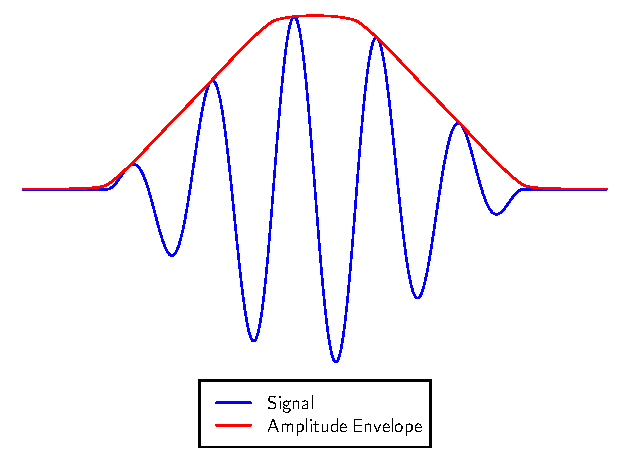
\includegraphics{chapter2/Images/AmplitudeEnvelope.pdf}
			\caption{The amplitude envelope of a signal.}
			\label{fig:AmplitudeEnvelope}
		\end{figure}

		\subsubsection*{Envelope Detection}
			Simple envelope detectors can be implemented based on those used in electronic circuits. First
			rectification is applied to produce a unipolar signal and then a low pass filter is applied to
			smooth the result \citep{dutilleux2011modulators}. In the digital domain more complex envelope
			detectors are possible such as the instantaneous amplitude detector. Instantaneous amplitude is
			calculated as the absolute value of an analytic representation of the input signal. An analytic
			signal is a complex valued signal, the real part of which is the original signal and the imaginary
			part its Hilbert transform. The analytic signal is often denoted with a subscript letter $a$, such
			that the analytic representation of the signal $x[n]$ would be denoted $x_{a}[n]$. This method and
			more complex digital envelope detectors are reviewed by \citet{chang2007a}. 

			Implementing an instantaneous amplitude detector involves making performance compromises. An ideal
			Hilbert transform alters the phase information of a signal while leaving the magnitude information
			unchanged. Any negative frequencies in the signal have their phase shifted by $\frac{\pi}{2}$
			radians while the phase of positive frequencies is shifted by $-\frac{\pi}{2}$ radians. The
			transfer function for an FIR implementation of a Hilbert transform is shown in
			Equation~\ref{eq:FirHilbertTransform}.

			\begin{equation}
				H(z) = \sum_{m = -M}^{M} \frac{2}{m\pi} sin^{2} \left( \frac{m\pi}{2} \right) z^{-m}
				\label{eq:FirHilbertTransform}
			\end{equation}

			For an ideal Hilbert transform the impulse response should be infinitely long ($M = \infty$).
			Practicable approximations of an ideal Hilbert transform can be created by using a finite value for
			$M$. A delay of $M$ samples must also be introduced in order to give a causal filter. As the value
			of $M$ is decreased this delay is reduced while the magnitude response of the filter deviates
			further from the ideal. Figure~\ref{fig:HilbertMagnitude} shows the magnitude responses for FIR
			Hilbert transform filters with $M = 11$ and $M = 101$. The filters have a bandpass response with
			some ripple in the pass band. As $M$ is increased the bandwidth of the passband is increased and
			the ripple reduced. The phase response of these filters remains ideal no matter the value of $M$,
			as evidenced by Figure~\ref{fig:HilbertPhase}.

			\begin{figure}[h!]
				\centering
				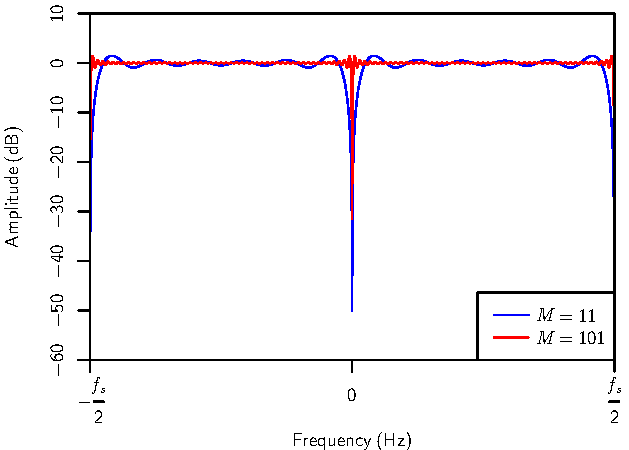
\includegraphics{chapter2/Images/HilbertMagnitudeResponses.pdf}
				\caption{Magnitude responses of FIR Hilbert transform filter with different orders.}
				\label{fig:HilbertMagnitude}
			\end{figure}

			\begin{figure}[h!]
				\centering
				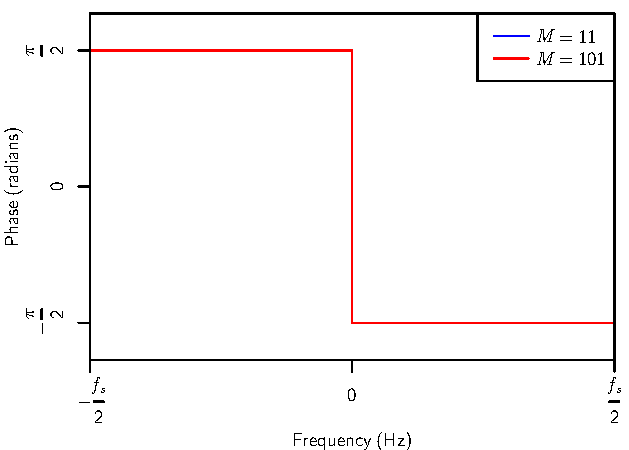
\includegraphics{chapter2/Images/HilbertPhaseResponses.pdf}
				\caption{Phase responses of FIR Hilbert transform filters with different orders.}
				\label{fig:HilbertPhase}
			\end{figure}

			When using Equation~\ref{eq:FirHilbertTransform} a compromise needs to be made between the
			tolerable amount of delay and the accuracy of the filter's magnitude response. Increasing $M$ will
			give a more accurate filter but introduce more delay and increase the complexity of the filter.
			More efficient implementations can be built using IIR filters if some of the properties of an ideal
			Hilbert transform are disregarded.  \citet{oppenheim2014discrete} suggest constructing a phase
			splitter: processing audio with two parallel allpass IIR filters the phase responses of which
			differ from each other by $\frac{\pi}{2}$ radians for a large proportion of the spectrum. While
			this is not strictly a Hilbert transform it creates two signals which can be used as the real and
			imaginary part of an analytic signal. \citet{niemitalo2003hilbert} provides an implementation of
			such a pair of filters. The phase difference between these two filters is seen in
			Figure~\ref{fig:IIRHilbertPhase}.

			\begin{figure}[h!]
				\centering
				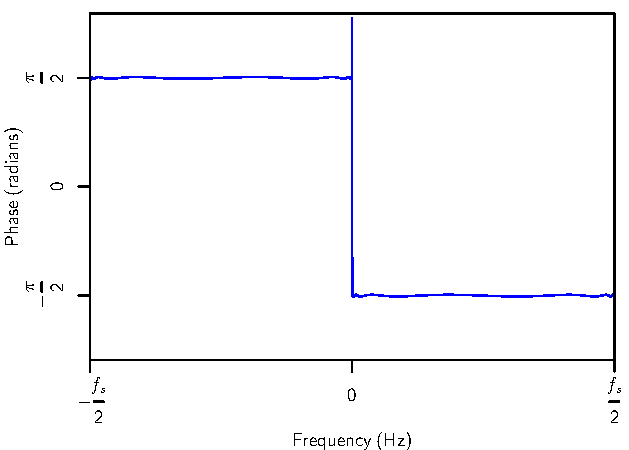
\includegraphics{chapter2/Images/IIRHilbertPhaseResponses.pdf}
				\caption{The phase difference between the two allpass filters proposed by
					 \citet{niemitalo2003hilbert}.}
				\label{fig:IIRHilbertPhase}
			\end{figure}

		\subsubsection*{Amplitude Envelope Analysis}
			The amplitude envelope of a signal can be used to extract more meaningful information about its
			temporal evolution. This is often done by splitting the sound into different sections according to
			the properties of its amplitude envelope. \citet{howard2009acoustics} separate the amplitude
			envelope of a sound into three sections: the steady state section being the middle portion in which
			the timbre of the sound only varies slightly and the onset and offset sections which describe the
			way the sound rises from silence to the steady state and returns to silence afterwards. Further
			refinement of the description of amplitude envelopes leads to the ADSR (Attack, Decay, Sustain,
			Release) model \citep{descrivan2012music}. The attack and decay portions constitute the onset of
			the signal, the attack describing the time it takes for the amplitude to rise from silence to a
			maximum and the decay describing the time it takes for the amplitude to decrease back to a steady
			level. The sustain describes the level at which the amplitude remains during the steady state
			portion of the signal and the release the time taken for the amplitude to fall from this level to
			silence. An example ADSR envelope is shown in Figure~\ref{fig:ADSR}.

			\begin{figure}[h!]
				\centering
				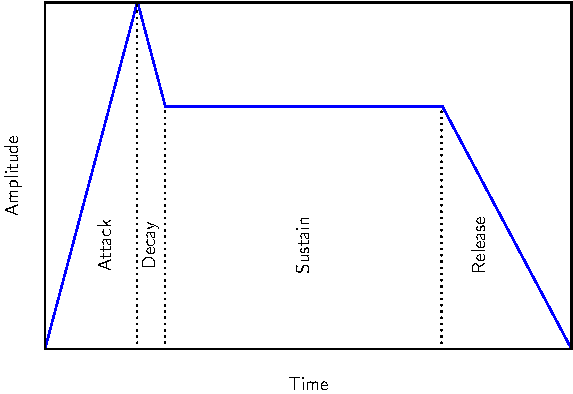
\includegraphics{chapter2/Images/ADSR.pdf}
				\caption{An ADSR envelope.}
				\label{fig:ADSR}
			\end{figure}

			Properties of the amplitude envelope can be used to describe the temporal features of a signal's
			amplitude. The attack time of sounds is important in the distinction of different timbres
			\citep{ilmoniemi2004subjective} and is often scaled logarithmically giving the log attack time.
			Other temporal features measure the amplitude envelope in its entirely, such as the temporal
			centroid which is the mean time of the signal's duration weighted by the amplitude at each instant
			\citep{peeters2000instrument}. The temporal evolution of the amplitude envelope can have a distinct
			effect on the perceived timbre of a sound. \citet{patterson1994the} show that signals with similar
			spectral content but different amplitude envelopes can be differentiated by listeners.

		\subsubsection*{Other Temporal Audio Features}
			Basic frequency information can be attained through temporal analysis by enumerating the number of
			specific events which happen in a given time period. One such event is a zero crossing (a change in
			signal polarity), the counting of which can yield an estimate of the frequency content of a signal
			(the zero crossing rate). The temporal distance between similar events in a signal can also be
			found through autocorrelation and used as an estimate of pitch / frequency \citep{mcleod2005a}.

			Features extracted from an amplitude envelope are used to describe the properties of individual
			notes produced by a source. As such they describe short portions of time; attack times typically
			being measured in milliseconds. Larger scale temporal features measure the properties of an entire
			passages of music rather than individual notes, such as the measure used by
			\citet{wilson2014profiling} in which the probability mass function (PMF) of sample amplitudes in a
			segment of audio is used as a measure of the distortion present in the signal.  Temporal features
			on this scale are outside of the scope of this work as they no longer relate to the timbre of
			individual sounds but rather the perceived nature of a musical piece.

	\subsection{Spectral Features}
	\label{sec:Timbre-LowLevelFeatures-Spectral}
		As stated by \cite{ASA1960american} the timbre of a sound is primarily influenced by its spectrum. In
		timbral research the properties of a signal's are summarised using a number of spectral features. To
		calculate these features the signal is first converted into a frequency domain representation. This is most
		commonly done using either the Discrete Fourier Transform (DTF) or a parallel filter bank. The calculation
		of many spectral features is done directly from these spectral representations; for others, peak finding is
		applied to the spectrum in order to determine the spectral partials.

		The spectral partials of a signal are its distinct frequency components. These are analogous to the
		vibrational modes of a physical body. Determining the spectral partials of a signal allows the tonal
		content of a signal to be isolated from the noise content. The noise energy in a signal describes any
		energy which does not contribute to a spectral partial. The noisiness of a signal can be measured as the
		ratio of the noise energy to the total energy in the signal \citep{serra1998sound}.

		Further analysis can be performed by finding the harmonic partials of the signal. This requires a
		calculation of the fundamental frequency ($f_{0}$) of the signal. $f_{0}$ is a property of periodic signals
		and is equal to the inverse of the signal's period (i.e. its lowest frequency component). Harmonic partials
		of a signal are the spectral partials with frequencies which are an integer multiple of the $f_{0}$. In
		detecting the harmonic partials it is usual to allow for a slight deviation from perfect harmonic
		structure, as described by \citet{peeters2011the}.

		To aid in discussion throughout this work it is useful to define the concept of a spectral component. This
		is a general concept used to describe individual portions of a signal's spectrum. A signal is composed of
		$N$ spectral components which are each described by an amplitude and a frequency. The amplitude and
		frequency of the $n$\super{th} spectral component are denoted $a_{n}$ and $\nu_{n}$ respectively. Spectral
		components can describe DFT bins, $a_{n}$ being the bin's magnitude and $\nu_{n}$ its frequency; filter
		bank bands, $a_{n}$ representing the total energy in the band and $\nu_{n}$ the band's center frequency; or
		spectral partials, $a_{n}$ and $\nu_{n}$ giving the amplitude and frequency of the partial. Several of the
		features discussed in this section can be calculated from any type of spectral components so this uniform
		notation proves very useful. Where the calculation of a feature requires a particular spectral
		representation this will be noted. Some features are calculated using only the energy at the harmonic
		frequencies of a signal. The equations for calculating these features use a slightly different notation.
		Features are calculated from the amplitudes of the first $N$ harmonics of a signal, the amplitude of the
		$n$\super{th} harmonic being denoted $h_{n}$. No additional notation is required for the frequency of the
		harmonic as it is implicitly equal to $nf_{0}$.

		\subsubsection*{Spectral Moments}
			The spectral moments are the statistical moments of a signal's spectrum. They describe how the
			energy is distributed in a spectrum. The first four spectral moments are the centroid, spread,
			skewness and kurtosis.

			The spectral centroid of a signal, $\mu_{\mathrm{s}}$, is the first raw moment (mean) of the
			spectrum. It is calculated using Equation~\ref{eq:SpectralCentroid}. Spectral centroid is often
			stated as being one of the most salient audio features in timbre recognition
			\citep{freed1990auditory, lakatos2000a}. 

			\begin{equation}
				\mu_{\mathrm{s}} = \frac{\sum_{n = 1}^{N} \nu_{n}a_{n}}
					   	   {\sum_{n = 1}^{N} a_{n}}
				\label{eq:SpectralCentroid}
			\end{equation}

			The spectral spread of a signal, $\sigma_{\mathrm{s}}^{2}$, is the second central moment (variance)
			of the spectrum. It is calculated using Equation~\ref{eq:SpectralSpread}.

			\begin{equation}
				\sigma_{\mathrm{s}}^{2} = \frac{\sum_{n = 1}^{N} a_{n}(\nu_{n} - \mu_{\mathrm{s}})^{2}}
						  	  {\sum_{n = 1}^{N} a_{n}}
				\label{eq:SpectralSpread}
			\end{equation}

			Together, the spectral centroid and spread give a description of where the energy in a spectrum is
			centered and how far from this center the energy is spread.

			The spectral skewness of a signal, $\gamma_{\mathrm{s}}$, is the third standardised moment of the
			spectrum. It is calculated using Equation~\ref{eq:SpectralSkewness}.

			\begin{equation}
				\gamma_{\mathrm{s}} = \frac{\sum_{n = 1}^{N} a_{n}(\nu_{n} - \mu_{\mathrm{s}})^{3}}
					{\sigma_{\mathrm{s}}^{3}\sum_{n = 1}^{N} a_{n}}
				\label{eq:SpectralSkewness}
			\end{equation}

			The spectral skewness measures how symmetrical a spectrum is about its centroid. A negative
			skewness describes a spectrum with more energy above its centroid while a positive skewness
			describes the opposite. A skewness of zero describes a spectrum with equal energy either side of
			its centroid.

			The spectral kurtosis of a signal, $\kappa_{\mathrm{s}}$, is the fourth standardised moment of the
			spectrum. It is calculated using Equation~\ref{eq:SpectralKurtosis}.

			\begin{equation}
				\kappa_{\mathrm{s}} = \frac{\sum_{n = 1}^{N} a_{n}(\nu_{n} - \mu_{\mathrm{s}})^{4}}
					{\sigma_{\mathrm{s}}^{4}\sum_{n = 1}^{N} a_{n}}
				\label{eq:SpectralKurtosis}
			\end{equation}

			The kurtosis measures the length of a distribution's tails. A low kurtosis describes a spectrum
			where the energy is evenly distributed in a band around the centroid. A high kurtosis describes a
			spectrum in which small amounts of energy lies at frequencies far away from the central band.

			The kurtosis of a normal distribution is 3. This gives rise to a different measure, the excess
			kurtosis, which is defined as $\kappa_{\mathrm{s}} - 3$. The excess kurtosis is often referred to
			as the kurtosis. This gives rise to some obscurity when reading literature which discusses the
			kurtosis without providing a definition.

		\subsubsection*{Spectral Irregularity}
			Spectral irregularity measures the smoothness of a magnitude spectrum. It is typically measured
			using the amplitudes of spectral partials as the spectra of pitched signals are characteristically
			`unsmooth', having sharp amplitude peaks at each partial. Various different methods of measuring
			this are often cited in the literature. The first being that proposed by
			\citet{krimphoff1994caracterisation}, shown in Equation~\ref{eq:KrimphoffIrregularity} and
			hereafter referred to as Krimphoff Irregularity ($\mathrm{KI}$).

			\begin{equation}
				\mathrm{KI} = \log_{10} \left( 20 \sum_{n = 2}^{N - 1}
						   \abs{\log_{10}(a_{n}) - \frac{\log_{10}(a_{n-1}a_{n}a_{n+1})}{3}}
						   \right)
				\label{eq:KrimphoffIrregularity}
			\end{equation}

			This is often implemented using the raw amplitudes of the partials rather than their dB amplitudes
			yielding Equation~\ref{eq:LibXtractKrimphoffIrregularity}. This is how the Krimphoff irregularity
			is implemented in LibXtract \citep{bullock2007libxtract} (a software library for audio analysis
			used throughout this work).

			\begin{equation}
				\mathrm{KI} = \sum_{n = 2}^{N - 1}
						  \abs{a_{n} - \frac{a_{n-1} + a_{n} + a_{n+1}}{3}}
				\label{eq:LibXtractKrimphoffIrregularity}
			\end{equation}

			A second method, Jensen irregularity ($\mathrm{JI}$), is proposed by \citet{jensen1999timbre},
			shown in Equation~\ref{eq:JensenIrregularity}.

			\begin{equation}
				\mathrm{JI} = \frac{\sum_{n = 1}^{N} (a_{n} - a_{n+1})^{2}}
						   {\sum_{n = 1}^{N} a_{n}^{2}},
					      \quad a_{N+1} = 0
				\label{eq:JensenIrregularity}
			\end{equation}

			A third method, Beauchamp irregularity ($\mathrm{BI}$) is given by \citet{beauchamp2007analysis},
			shown in Equation~\ref{eq:BeauchampIrregularity}.

			\begin{gather}
			        \bar{a}_{n} = \frac{a_{n-1} + a_{n} + a_{n+1}}{3} \nonumber \\
				\mathrm{BI} = \frac{\sum_{n = 2}^{N - 1} \bar{a}_{n} \abs{a_{n} - \bar{a}_{n}}}
						   {\sum_{n = 2}^{N - 1} \bar{a}_{n} \sqrt{\sum_{n = 1}^{N} a_{n}^{2}}}
				\label{eq:BeauchampIrregularity}
			\end{gather}

			Equation \ref{eq:JensenIrregularity} and \ref{eq:BeauchampIrregularity} have an advantage over
			Equations \ref{eq:KrimphoffIrregularity} and \ref{eq:LibXtractKrimphoffIrregularity} in that they
			produce normalised values. Equation~\ref{eq:JensenIrregularity} produces values between zero and
			two while Equation~\ref{eq:BeauchampIrregularity} produces values between zero and one. This allows
			measures of irregularity of two different signals to be compared more easily.

		\subsubsection*{Spectral Flatness}
			Spectral flatness, $\mathrm{SF}$, measures how uniformly distributed the energy is in the spectrum.
			\citet{johnston1988transform} measures the spectral flatness as the ratio of the geometric and
			arithmetic means of the power spectrum of a signal (Equation~\ref{eq:Flatness}).

			\begin{equation}
				\mathrm{SF} = \frac{N\sqrt[N]{\prod_{n = 1}^{N} a_{n}^{2}}}
						   {\sum_{n = 1}^{N} a_{n}^{2}}
				\label{eq:Flatness}
			\end{equation}

			The arithmetic and geometric means of any list of $N$ non-negative numbers, $L$, satisfy the
			inequality in Equation~\ref{eq:MeanInequality}.

			\begin{equation}
				\sqrt[N]{\prod_{n = 1}^{N} L_{n}} \leq \frac{1}{N} \sum_{n = 1}^{N} L_{n}
				\label{eq:MeanInequality}
			\end{equation}

			Where $L_{n}$ is the $n$\super{th} element of list $L$. The two means are only equal if all
			elements of $L$ have the same value.

			Due to this, the spectral flatness of a signal takes a value between zero and one. Low values
			describe signals whose energy lies in narrow bands of the spectrum (tones). High values describe
			signals whose energy is more spread out, a value of one describing a signal where all bins of the
			power spectrum have the same amplitude (white noise). This means the spectral flatness also gives a
			description of the tonality / noisiness of a signal.

			The spectral flatness is traditionally measured using DFT bins as spectral components. This way any
			signal which has zero energy in any DFT bin will produce a spectral flatness of zero. Musical
			signals which are composed of a set of frequency partials may have areas of the spectrum with zero
			energy. Several different sounds with radically different spectral envelopes can then all exhibit a
			spectral flatness of zero. This is particularly problematic for digitally synthesised signals as
			they do not have the inherent noise present in recorded sounds. The method used by
			\citet{peeters2004a} mitigates this by using filter bank bands as the spectral components. It is
			less likely that there will be zero energy in a wider spectral band than a single DFT bin. Another
			method to avoid spectral flatnesses of zero is to use the signals partials as spectral components.
			This no longer measures the tonality / noisiness of a signal but rather the flatness of its
			spectral envelope.

		\subsubsection*{Spectral Slope}
			The spectral slope, $\mathrm{SSl}$ measures the gradient of the spectrum. It is calculated by first
			order liner regression of the spectrum. For a signal with $N$ spectral components the spectral
			slope can be calculated with Equation~\ref{eq:SpectralSlope}.

			\begin{gather}
				A = \sum_{n = 1}^{N} a_{n}
				\quad 
				B = \sum_{n = 1}^{N} \nu_{n}a_{n} \nonumber \\
				F = \sum_{n = 1}^{N} \nu_{n} \quad G = \sum_{n = 1}^{N} \nu_{n}^{2} \nonumber \\
				\mathrm{SSl} = \frac{1}{A} \frac{NB - FA}{NG - F^{2}}
				\label{eq:SpectralSlope}
			\end{gather}

			Negative values of spectral slope describe a spectrum where the majority of the energy is in the
			low end of the spectrum. Positive values describe signals with more energy in the high end of the
			spectrum. Traditional measures of spectral slope are calculated using the amplitudes and
			frequencies of the DFT bins. For musical signals which are composed of partials it may be more
			beneficial to measure the slope of the partial's amplitudes rather than of the whole spectrum. 
			
			Equation~\ref{eq:SpectralSlope} produces values with units of Hz\super{-1}. The equation can be
			altered to provide results in units of dB per Hz by substituting $a_{n}$ with $20\log_{10}(a_{n})$
			and removing the scaling factor of $\frac{1}{A}$ from the final calculation, giving
			Equation~\ref{eq:SpectralSlope2}.
			
			\begin{gather}
				A = \sum_{n = 1}^{N} 20\log_{10}(a_{n})
				\quad 
				B = \sum_{n = 1}^{N} 20\nu_{n}\log_{10}(a_{n}) \nonumber \\
				F = \sum_{n = 1}^{N} \nu_{n} \quad G = \sum_{n = 1}^{N} \nu_{n}^{2} \nonumber \\
				\mathrm{SSl} = \frac{NB - FA}{NG - F^{2}}
				\label{eq:SpectralSlope2}
			\end{gather}
			
			A commonly used unit for measuring slopes in spectra is dB per octave, as used when measuring the
			roll off rate in a filters stop band. Equation~\ref{eq:SpectralSlope2} can be altered to produce
			values in this unit by substituting $\nu_{n}$ with $\log_{2}(\nu_{n})$.

		\subsubsection*{Tristimulus}
			The tristimulus metrics, $T_{1}$, $T_{2}$ and $T_{3}$, are a set of three metrics proposed by
			\citet{pollard1982a} which measure the distribution of energy in a signal's spectrum. They are
			calculated using the harmonic partials of a signal by use of Equations \ref{eq:Tristimulus1},
			\ref{eq:Tristimulus2} and \ref{eq:Tristimulus3}.
			
			\begin{equation}
				T_{1} = \frac{h_{1}}{\sum_{n = 1}^{N} h_{n}}
				\label{eq:Tristimulus1}
			\end{equation}

			\begin{equation}
				T_{2} = \frac{h_{2} + h_{3} + h_{4}}{\sum_{n = 1}^{N} h_{n}}
				\label{eq:Tristimulus2}
			\end{equation}

			\begin{equation}
				T_{3} = \frac{\sum_{n = 5}^{N} h_{n}}{\sum_{n = 1}^{N} h_{n}}
				\label{eq:Tristimulus3}
			\end{equation}

			Each tristimulus metric measures the amplitude ratio of a specific set of harmonics and all the
			harmonics. In each of these equations the denominator is always greater than or equal to the
			numerator, meaning the tristimulus takes values from zero to one. Zero meaning there is no energy
			in that set of harmonics, one meaning the signal is entirely composed of those harmonics.

			In this work a generalisation of the tristimulus metrics is proposed which includes the inharmonic
			partials of a signal. These are called the peak tristimulus measures ($T_{\mathrm{p}1}$,
			$T_{\mathrm{p}2}$ and $T_{\mathrm{p}3}$) and give a measure analogous to the tristimulus which can
			be used on more inharmonically structured signals. The spectrum is still split into three bands but
			the number of partials within these bands depends on the content of the signal. The bands include
			all partials with a frequency within $0.5f_{0}$Hz of the harmonics in the equivalent band used in
			the calculation of tristimulus.  The peak tristimulus measures are given by Equations
			\ref{eq:PeakTristimulus1}, \ref{eq:PeakTristimulus2} and \ref{eq:PeakTristimulus3}.

			\begin{gather}
				P = \left\{ n | n \in \textbf{N} \land n \leq N \right\} \nonumber \\
				F = \left\{ n | n \in P \land 0.5f_{0} \leq \nu_{n} < 1.5f_{0} \right\} \nonumber \\
				T_{\mathrm{p}1} = \frac{\sum_{n \in F} a_{n}}{\sum_{n = 1}^{N} a_{n}}
				\label{eq:PeakTristimulus1}
			\end{gather}

			\begin{gather}
				M = \left\{ n | n \in P \land 1.5f_{0} \leq \nu_{n} < 4.5f_{0} \right\} \nonumber \\
				T_{\mathrm{p}2} = \frac{\sum_{n \in M} a_{n}}{\sum_{n = 1}^{N} a_{n}}
				\label{eq:PeakTristimulus2}
			\end{gather}

			\begin{gather}
				H = \left\{ n | n \in P \land \nu_{n} \geq 4.5f_{0} \right\} \nonumber \\
				T_{\mathrm{p}3} = \frac{\sum_{n \in H} a_{n}}{\sum_{n = 1}^{N} a_{n}}
				\label{eq:PeakTristimulus3}
			\end{gather}

		\subsubsection*{Odd to Even Harmonic Ratio}
			The odd to even harmonic ratio, $\mathrm{OER}$, measures the ratio of energy between odd and even
			order harmonics in a signal. It was found to be a salient feature in timbral recognition by
			\citet{hall2010importance}, allowing for distinction between signals which consist of only a single
			parity of harmonic. The ratio is calculated from the squared amplitudes of the harmonic partials in
			a signal according to Equation~\ref{eq:HarmonicParityRatio}.
			
			\begin{equation}
				\mathrm{OER} = \frac{\sum_{1 \leq n \leq N, n \text{ is odd}} h_{n}^{2}}
					       {\sum_{1 \leq n \leq N, n \text{ is even}} h_{n}^{2}}
				\label{eq:HarmonicParityRatio}
			\end{equation}

			Measuring the $\mathrm{OER}$ of a signal using Equation~\ref{eq:HarmonicParityRatio} produces an
			asymmetric scale which may be difficult to interpret.  Signals with most of their energy at even
			harmonics produce values between zero and one.  Signals with more energy at the odd harmonics can
			produce any value greater then one. Another problem arises for signals with no energy at even
			harmonics where a division by zero will occur. A more robust method is to use separate measures for
			the proportion of odd harmonics in a signal and the proportion of even harmonics in a signal.
			\citet{lukasik2005towards} describes two metrics which measure the oddness, $O$, and the evenness,
			$E$, of a signal producing more easily interpreted values of 0 and 1. Formulae for the oddness and
			evenness are given in Equations \ref{eq:Oddness} and \ref{eq:Evenness}.

			\begin{equation}
				O = \sqrt{\frac{\sum_{1 \leq n \leq N, n \text{ is odd}} h_{n}^{2}}
					       {\sum_{n = 1}^{N} h_{n}^{2}}}
				\label{eq:Oddness}
			\end{equation}

			\begin{equation}
				E = \sqrt{\frac{\sum_{1 \leq n \leq N, n \text{ is even}} h_{n}^{2}}
					       {\sum_{n = 1}^{N} h_{n}^{2}}}
				\label{eq:Evenness}
			\end{equation}

		\subsubsection*{Inharmonicity}
			Inharmonicity, $I$, is a measure of how much the frequencies of a signal's partials deviate from
			harmonic frequencies. As such it must be calculated from the amplitudes and frequencies of a
			signal's spectral partials. \citet{fletcher1962quality} state that inharmonicity of some partials
			is necessary for the recognition of the timbre of a piano. The inharmonicity of a signal is
			measured using Equation~\ref{eq:Inharmonicity}.
			
			\begin{equation}
				I = \frac{2\sum_{n = 1}^{N}a_{n}^{2}
					   \abs{\nu_{n} - f_{0}\round{\frac{\nu_{n}}{f_{0}}}}}
					   {f_{0}\sum_{n = 1}^{N} a_{n}^{2}}
				\label{eq:Inharmonicity}
			\end{equation}

			This produces values between zero and one. Zero describing a signal in which all partials have
			perfectly harmonic frequencies and one describing a signal where all partials have frequencies
			lying $\frac{f_{0}}{2}$Hz from harmonic frequencies.

\section{Psychoacoustic Principles}
\label{sec:Timbre-PsychoacousticPrinciples}
	As discussed in the previous section, there are several metrics which describe the low level features of audio
	signals. While it is possible to measure changes in the values of these features, these changes may not be
	detectable by or linearly related to the human hearing system. To understand the possible effects an audio feature
	can have on perceived timbre we must model how that feature itself is perceived. Several models have been proposed
	by research in psychoacoustics, a field which studies the perception of sound. The existing psychoacoustic
	literature concerns the study of the human hearing system and how it responds to certain aspects of audio stimuli.
	Several different areas of audio perception have been researched. Methods have been devised to model the human
	perception of loudness \citep{moore1997a} and pitch \citep{gerhard2003pitch}. Other research considers the human
	hearing system's ability to locate sound sources \citep{blauert1997spatial}. This section covers the key principles
	of psychoacoustics relevant to this work.

	\subsection{Psychoacoustic Frequency}
	\label{sec:Timbre-PsychoacousticPrinciples-Frequency}
		In scientific work frequency is typically discussed as an absolute number of cycles per second in units of
		Hertz. In music theory the frequency difference between two sounds is described in terms of tones and
		octaves.  This musical notation assumes that the ratio of two frequencies defines the perceived interval
		between them: the perceived difference between 50 and 75Hz is the same as that between 1kHz and 1.5kHz.
		While this model suffices for musical composition and performance it does not accurately describe the
		perception of frequency by human listeners. \citet{stevens1937a} propose a new frequency scale, the mel
		scale, on which a given change in frequency produces the same perceived interval. This scale was devised
		through a series of listening tests in which participants were asked to adjust the frequency of a tone such
		that it had a pitch which was half that of a reference tone. This was repeated for ten individual reference
		tones producing ten data points which were used to provide a mapping between the hertz and mel scales. A
		formula to approximate the frequency in mel, $m$, for any given frequency in hertz, $f$, is given by
		\citet{oshaughnessy2000speech} (Equation~\ref{eq:mel}), shown graphically in Figure~\ref{fig:MelScale}.

		\begin{equation}
			m = 2595 \log_{10} \left(1 + \frac{f}{700} \right)
			\label{eq:mel}
		\end{equation}

		\begin{figure}[h!]
			\centering
			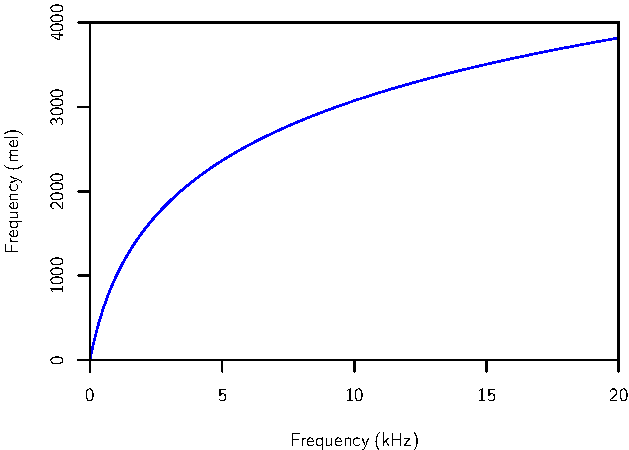
\includegraphics{chapter2/Images/MelScale.pdf}
			\caption{The mel frequency scale.}
			\label{fig:MelScale}
		\end{figure}

		This perceptual frequency scale allows audio feature metrics to analyse audio in more perceptually relevant
		bands. One such metric is the Mel Frequency Cepstral Coefficients (MFCCs) developed for use in speech
		recognition \citep{davis1980comparison}. These provide more detailed information about the shape of the
		spectrum than the spectral moments discussed in Section~\ref{sec:Timbre-LowLevelFeatures-Spectral}. In
		brief the power spectrum of a signal is partitioned into bands which are equally spaced on the mel scale.
		The discrete cosine transform (DCT) of the log powers of these bands is then calculated to produce the
		MFCCs. From their first use in speech recognition MFCCs have been added to the corpus of audio features
		used by researchers investigating timbre \citep{depoli1997sonological}. 

		Investigating the perception of frequency allows us to build models of how the human hearing system detects
		and processes frequency information. This not only allows for the description of the perception of
		individual tones but also the perception of tones played simultaneously. In certain situations a sound will
		mask the perception of another sound, causing it to become inaudible. The degree of masking between two
		sounds depends on the amplitude, frequency and temporal relationships between them. Two sounds which are
		perceptually close in frequency are more likely to perceptually interact with each other causing one to be
		masked. More detailed examination of the human hearing system reveals the maximum difference in frequency
		between two tones for which masking will occur, the critical bandwidth.

	\subsection{Critical Bands}
	\label{sec:Timbre-PsychoacousticPrinciples-CriticalBands}
		The part of the inner ear that deals with frequency separation is known as the basilar membrane. This is a
		structure which resonates at different frequencies along its length; low frequencies at one end to high at
		the other. A sinusoidal tone excites a portion of the basilar membrane corresponding to a narrow band of
		frequencies. A tone whose excitation band overlaps with another will interfere with how the other tone is
		perceived by a listener. The basilar membrane can be modelled as a parallel filter bank comprised of band
		pass filters, each of these auditory filters representing the region of the membrane excited by a
		sinusoidal tone at its centre frequency. The bandwidth of these filters is known as the critical bandwidth.
		Portions of signals will interfere with the perception of others which are within one critical bandwidth.
		\citet{glasberg1990derivation} simplify the auditory filters by modelling them as rectangular filters. The
		bandwidth of these filters known as the equivalent rectangular bandwidth ($\mathrm{ERB}$) and can be
		approximated using Equation~\ref{eq:ERB}.

		\begin{equation}
			\mathrm{ERB}(f_{c}) = 24.7(4.37f_{c} + 1)
			\label{eq:ERB}
		\end{equation}

		Where $f_{c}$ is the center frequency of the auditory filter in kHz and $\mathrm{ERB}(f_{c})$ is the
		equivalent rectangular bandwidth, in Hz, at that frequency.

		\citet{howard2009acoustics} discusses the perception of two tones played simultaneously as they get further
		apart in frequency. When within 15Hz of one another the two tones are perceived as a single sound with a
		sinusoidally varying amplitude. The frequency of this variation is equal to the difference in frequency
		between the tones. As the difference in frequency increases beyond 15Hz this amplitude modulation becomes
		fast enough for it to be perceived as a roughness in texture rather than `beats' in the amplitude. In
		between 15Hz and the critical bandwidth the perceived sound transitions from a single sound to two separate
		sounds but still with a rough texture. Once the difference in frequency exceeds the critical bandwidth the
		two tones are perceived as separate tones. These effects are summarised in Figure~\ref{fig:ToneSeparation}.

		\begin{figure}[h!]
			\centering
			\begin{tikzpicture}

				\draw [thick, ->] (0, 0) -- (10, 0);
				\draw (0, 1) -- (10, 1);
				\draw (0, 0) -- (0, 2) -- (10, 2);

				\draw (0, 0) -- (0, -2pt) node [anchor=north] {0};
				\draw (2, 0) -- (2, -2pt) node [anchor=north] {15};
				\draw (8, 0) -- (8, -2pt) node [anchor=north] {CB};

				\fill [pattern=north west lines] (1.75, 0) rectangle (2.25, 1);
				\fill [pattern=north west lines] (7.75, 0) rectangle (8.25, 1);
				\fill [pattern=north west lines] (5.75, 1) rectangle (6.25, 2);

				\node at (0.875, 0.5) {Beats};
				\node at (5, 0.5) {Rough};
				\node at (9.125, 0.5) {Smooth};
				\node at (2.875, 1.5) {Fused};
				\node at (8.125, 1.5) {Separate};

				\node at (5, -1) {Frequency Difference (Hz)};

			\end{tikzpicture}
			\caption{The perception of two tones as they move further apart in frequency. Hashed areas
				 represent the transition between perceived effects. CB denotes the critical bandwidth.}
			\label{fig:ToneSeparation}
		\end{figure}

		It is evident from Equation~\ref{eq:ERB} that the critical bandwidth increases with frequency. This,
		together with the perceptual information shown in Figure~\ref{fig:ToneSeparation}, suggests that tones
		separated by the same amount will be heard as separate if they are both low in frequency but as their
		frequencies rise they will start to be perceived as a single fused sound.

	\subsection{Specific Loudness}
	\label{sec:Timbre-PsychoacousticPrinciples-SpecificLoudness}
		In hearing models for measuring loudness it is common to split the audible spectrum into bands which all
		have the same perceived width. The specific loudness measures the perceived loudness of a signal in each of
		these bands. For the analysis of the perception of timbre this allows for better modelling of what portions
		of a signal's spectrum are audible. While the spectrum describes what frequency content is present in the
		signal, the specific loudness describes how much of each frequency is perceived by a listener.  The total
		loudness of a signal is calculated as the sum of the specific loudnesses of each frequency band. The full
		procedure for calculating loudness is beyond the scope of this work, a description of the process is
		provided by \citet{moore1997a}. 

		A widely used set of psychoacoustically spaced frequency bands was proposed by
		\citet{zwicker1961subdivision} who spilt the spectrum into 24 parts, each one critical bandwidth wide.
		These bands are known as the bark bands and provide another perceptual unit of frequency, the bark. Integer
		values of barks occur at the boundaries between two bark bands. A change in frequency of one bark is equal
		to one critical bandwidth.

\section{Psychoacoustic Models of Timbral Descriptors}
\label{sec:Timbre-TimbralFeatures}
	One method of relating semantic descriptors to measurable features of an audio signal is through the use of
	psychoacoustic models. To construct these, a semantic descriptor is chosen and a hypothesis made as to what
	attributes of a signal it describes. Psychoacoustic principles are then used to formulate a model describing how
	these attributes are interpreted by the human hearing system. This model is then refined through listening
	experiments so that the resulting metric is proportional to perception of the attribute it describes. As the
	features relating to a description are hypothesised, models can only be built in this manner for descriptors which
	are known to describe particular phenomena. There are two such descriptors which have received considerable
	attention in previous research: sharpness, describing the unpleasant nature of high frequency sounds; and
	roughness, used to describe the dissonance of particular musical intervals. Proposed psychoacoustic models for
	these descriptors are given in this section.
	
	\subsection{Sharpness}
	\label{sec:Timbre-TimbralFeatures-Sharpness}
		\citet{fastl2007psychoacoustics} discuss the factors leading to the perception of sharpness. The sharpness
		of a signal depends on the ratio of high and low frequency content. Increasing the amount of high frequency
		content increases the sharpness of a signal. The sharpness can also be reduced by adding more low frequency
		content to a signal. They produce a metric from this information for the measurement of perceived
		sharpness. The sharpness, $S$, is calculated using Equation~\ref{eq:Sharpness}.

		\begin{equation}
			S = 0.11\frac{\sum_{b = 1}^{24} N'_{b}g(b)b}{\sum_{b = 1}^{24}N'_{b}}
			\label{eq:Sharpness}
		\end{equation}

		Where $N'$ is the specific loudness of bark band $b$ and $g(b)$ is a weighting function designed to
		emphasise the presence of high frequency content.

		\citet{marui2006predicting} ran listening experiments to test how well perceived sharpness can be predicted
		using this metric. They find that it does not predict the sharpness of broadband noise accurately and
		propose an improved metric which is the product of the value from Equation~\ref{eq:Sharpness} and the
		spectral variance of the specific loudness.

	\subsection{Roughness}
	\label{sec:Timbre-TimbralFeatures-Roughness}
		A sensation of roughness was discussed in Section~\ref{sec:Timbre-PsychoacousticPrinciples-CriticalBands}.
		Here the roughness was due to the rapid amplitude modulation produced as a result of summing two sinusoids
		which are close in frequency. Much early research into this effect (summarised by \citet{plomp1965tonal})
		concerns the study of consonance or dissonance of tones, concluding that dissonance is manifested as a
		sensation of roughness due to amplitude fluctuations. They also suggest a relationship to critical
		bandwidth, stating that the most dissonant (roughest) interval between tones is one quarter of the critical
		bandwidth. \citet{vassilakis2010psychoacoustic} suggest that the sensation of roughness depends on more of
		the attributes of a signal, listing four characteristics:

		\begin{itemize}
			\item The signal intensity.
			\item The magnitude of the amplitude fluctuation.
			\item The frequency of the amplitude fluctuation.
			\item The frequency of the modulated signal.
		\end{itemize}

		Using these criteria a method is proposed for calculating the roughness of a signal consisting of two
		sinusoidal tones. Where $a_{1}$ and $\nu_{1}$ represent the amplitude and frequency of the lowest frequency
		tone and $a_{2}$ and $\nu_{2}$ those of the highest, the roughness, $R$, is calculated using
		Equation~\ref{eq:PartialRoughness}.
		
		\begin{gather}
			X = a_{1}a_{2} \nonumber \\
			Y = 2\frac{\min(a_{1}, a_{2})}{a_{1} + a_{2}} \nonumber \\
			s = \frac{0.24}{0.0207\nu_{1} + 18.96} \nonumber \\
			Z = e^{-3.5s(\nu_{2} - \nu_{1})} - e^{-5.75s(\nu_{2} - \nu_{1})} \nonumber \\
			R = 0.5X^{0.1}Y^{3.11}Z
			\label{eq:PartialRoughness}
		\end{gather}

		The intermediate variables in this equation model the different dependencies of roughness: $X$ modeling the
		dependence on signal intensity, $Y$ the dependence on the magnitude of the amplitude fluctuation and $Z$
		the dependence on the frequency of the signal and the amplitude fluctuation. The roughness of more complex
		tones can be calculated as the sum of the roughnesses of each pair of tones within the signal. 
		
		The frequency dependence of this model agrees with that shown in Figure~\ref{fig:ToneSeparation}. Amplitude
		fluctuations above approximately 15Hz produce a rough texture to the sound. As this frequency increases the
		roughness also increases to a maximum before decreasing again. At some frequency between 75Hz and 150Hz,
		depending on the frequency content of the modulated signal, the sensation of roughness ceases to be
		audible.

		The constants used in Equation~\ref{eq:PartialRoughness} were arrived at through experimentation, while the
		researchers report high correlations with perceived roughness this may not model all the possible
		interactions of tones within the human hearing system. \citet{fastl2007psychoacoustics} use the same four
		criteria to develop a different model of roughness, including more detailed modelling of auditory masking.
		This model takes account of both simultaneous masking (tones played simultaneously interfering with one
		another) and temporal masking (tones played close together in time interfering with one another). A full
		discussion of this model is beyond the scope of this report.

\section{Subjective Listening Tests}
\label{sec:Timbre-ListeningTests}
	The psychoacoustic models presented in the previous section are restricted to modelling descriptors for which
	informal definitions are already widely used. To investigate other aspects of timbre subjective listening tests
	must be carried out in order to collect information about the perception of sound. Depending on the nature of the
	experiment there are several different testing methodologies which have been proposed \citep{bech2006perceptual}.
	Those most prevalent in timbral research will be discussed here.

	\subsection{Testing Methodologies for Timbral Analysis}
	\label{sec:Timbre-ListeningTests-Methods}
		Two different classes of listening test are common in timbral studies. In one, participants are asked to
		judge the dissimilarity of small sets of audio stimuli. In the other, participants are asked to rate each
		audio stimulus on various scales which relate to attributes of the timbre. In this report, these methods
		will be referred to as dissimilarity tests and attribute scale tests respectively.

		\subsubsection*{Dissimilarity Tests}
			\citet{grey1977multidimensional} utilises a pairwise dissimilarity methodology to gather similarity
			data about audio stimuli. Participants are asked to rate the similarity of pairs of audio stimuli.
			Pairs of stimuli are presented one at a time until every possible pair from the set of stimuli has
			been rated. This is a popular method as it ensures that the participants rate every stimulus
			against every other stimulus. A downside of this is that the number of possible pairs grows
			exponentially as the total number of stimuli increases. This causes the time taken to complete the
			test to become practically too large if the experimenter wishes to evaluate a large corpus of
			stimuli.

			\citet{caclin2005acoustic} also use a pairwise dissimilarity method but unlike
			\citet{grey1977multidimensional} use synthetic stimuli rather than acoustically recorded ones. This
			allows them to better control the differences between them. All stimuli in their experiment only
			differed in three characteristics (attack time, spectral centroid and spectral flux) allowing them
			to identify which factors these features contribute to the timbre of a sound.

			Another method of capturing similarity data is that of triadic comparisons
			\citep{wickelmaier2007deriving}. In this method audio stimuli are presented in triads (three at a
			time). Participants are asked to identify the most similar pair of stimuli in the triad as well as
			the least similar. This method helps remove inconsistent use of a rating scale. In pairwise
			dissimilarity tests, participants may reinterpret the range of the scale they are given to rate
			dissimilarity on during the experiment. Triadic comparison asks which pair is most similar and
			which is the least, avoiding the elicitation of a value on a scale.

			Another popular testing technique is to carry out multiple stimulus tests. In a multiple stimulus
			test participants are presented with several stimuli simultaneously and asked to rate each against
			a given criteria. A multiple stimuli methodology often used in perceptual audio tests is MUSHRA
			(Multiple Stimuli with Hidden Reference and Anchor) \citep{mushra2014}. MUSHRA was developed for
			grading the quality of lossy audio data compression algorithms. Participants presented with several
			compressed versions of a signal simultaneously and asked to grade how similar each of them are to a
			reference signal (the uncompressed version) on a scale from 0 to 100. Among the signals to be
			graded are a hidden reference and anchor which are used to evaluate the reliability of a
			participants results. The hidden reference is the same as the reference signal and as such should
			be given a grade of 100. The anchor is a low pass filtered version of the signal, processed such
			that it is less similar to the reference than any of the compressed signals and hence should
			receive the lowest grade. Results are deemed reliable if they correctly identify the hidden
			reference (grading to 100) and anchor (giving it the lowest grade). These tests are often used to
			assess the performance of bandwidth extension methods such as those discussed in
			Section~\ref{sec:Excitation-Methods}. Other multiple stimulus tests, while not adhering strictly to
			the MUSHRA guidelines, follow a similar structure.  \citet{arthi2015influence} use a multiple
			stimulus test to determine the perceptual differences between stimuli. 
			
			Dissimilarity tests can provide accurate information about the perceived differences between
			timbres, allowing for similar timbres to be graded or classified into groups. No information,
			however, is gathered about how participants might describe the timbres of these groups and
			the differences in timbre between groups. An additional stage to the listening test is required in
			order to attribute descriptors to describe the timbres of the stimuli. If the description of timbre
			is an important outcome of the experiment an attribute scale test may be more suitable.
			
		\subsubsection*{Attribute Scale Tests}
			Attribute scale tests require participants to rate each stimulus against several scales which each
			relate to an attribute of their timbre. This is often done using a set of semantic differentials (a
			scale with opposing descriptors on each end). This is popular for timbral research as it provides
			rankings of audio stimuli against timbral descriptors. This not only allows for inference of the
			perceptual differences between stimuli but also for descriptors to be applied to describe these
			differences as done by \citet{zacharakis2014an}. 			
			
			In an attribute scale test the stimuli are presented to the participants one at a time and rated
			against several criteria. This is in direct opposition to a multiple stimulus test in which the
			stimuli are all presented at once and rated against a single criteria. Attribute scale tests pose a
			problem here as there is no reference provided against which to rate the stimuli. Participants must
			keep several scales (one for each descriptor) in mind throughout the duration of the test. This may
			cause them to use the extremes of the scales too early in the test so when presented with a
			stimulus they wish to rate closer to the extremes they cannot. In a multiple stimulus test all the
			stimuli being compared are available at once, allowing participants to find the stimuli which lie
			at the extremes and rate the rest accordingly. This better utilises the range of the scale. 
			
			Issues with the use of semantic differentials were shown by \citet{kendall1993verbal1}. Their first
			experiment was an attribute scale test in which participants are asked to rate each audio stimulus
			on eight different bipolar adjective scales, shown in Table~\ref{tab:vonBismarcksDescriptors}.

			\begin{table}[h!]
				\centering
				\begin{tabular}{|c|C{3cm}cC{3cm}|}
					\hline
					\bf{No.} & \multicolumn{3}{c|}{\bf{Adjectives}} \tabularnewline
					\hline
					\hline
					1 & hard & $\Longleftrightarrow$ & soft \tabularnewline
					\hline
					2 & sharp & $\Longleftrightarrow$ & dull \tabularnewline
					\hline
					3 & loud & $\Longleftrightarrow$ & soft \tabularnewline
					\hline
					4 & complex & $\Longleftrightarrow$ & simple \tabularnewline
					\hline
					5 & compact & $\Longleftrightarrow$ & scattered \tabularnewline
					\hline
					6 & pure & $\Longleftrightarrow$ & mixed \tabularnewline
					\hline
					7 & dim & $\Longleftrightarrow$ & brilliant \tabularnewline
					\hline
					8 & heavy & $\Longleftrightarrow$ & light \tabularnewline
					\hline
				\end{tabular}
				\caption{Bipolar adjectives scales used by \citet{kendall1993verbal1}.}
				\label{tab:vonBismarcksDescriptors}
			\end{table}

			They propose that semantic differential tests have a problem in that the descriptors at each end of
			the bipolar scales may not be the semantic opposites of each other. The difference between hard and
			soft, for instance, may not be a simple one dimensional relationship. In order to determine the
			effect of this they proposed the Verbal Attribute Magnitude Estimation (VAME) method in which the
			opposites of the adjectives were merely their negation (hard $\Leftrightarrow$ not hard, sharp
			$\Leftrightarrow$ not sharp etc.). This was found to increase the independence between each
			adjective scale in the ratings given by participants. 

			Attribute scale methods have an advantage over dissimilarity tests as they gather information about
			which aspects of the stimuli the participants are judging. A major disadvantage however is that non
			of the stimuli are directly compared against one another. The participants have no reference of
			where they have put other stimuli on the adjective scales making it difficult to use the scales
			consistently. \citet{marui2005constructing} uses both a semantic differential test and triadic
			comparisons in order to avoid the weaknesses of both methodologies. 

			A difficulty encountered when designing an attribute scale test is the selection of descriptors to
			use in the tests. As discussed by \citet{darke2005assessment}, results are not usable if the test
			participants find it difficult to associate a particular descriptor with the audio stimuli
			presented. The adjectives need to be meaningful to the test participants and also applicable to the
			audio stimuli used. The adjectives are often selected using a preliminary verbal elicitation
			experiment. \citet{namba1991verbal} presented participants with the test stimuli in a random order
			and asked them to provide any terms they would use to describe them. These terms were then used as
			the adjectives for the test. The adjectives used by \citet{kendall1993verbal1}, shown in
			Table~\ref{tab:vonBismarcksDescriptors} were taken from earlier work performed by
			\citet{vonbismarck1974timbre}. In a second set of experiments \citet{kendall1993verbal2} use a
			different set of adjectives taken from work on orchestration for composition
			\citet{piston1955orchestration}. The selection of adjectives was further refined through a simple
			elicitation experiment in which participants were asked to select those which were most applicable
			to the audio stimuli. It is reported that using this method produces better results in the timbral
			experiment than when the adjectives were selected by the experimenter.

	\subsection{Testing Environments}
	\label{sec:Timbre-ListeningTests-Environments}
		Once a testing methodology has been chosen, the task remains to recruit participants and have them
		undergo the test. Perceptual audio tests necessarily involve the use of audio reproduction equipment and a
		means of recording the participants' responses. The reproduction system and response method chosen has
		impacts on the reliability of the results and the sample size of participants. Two common approaches are to
		run supervised listening tests with specific reproduction equipment in a laboratory, or to produce a web
		interface to the experiment allowing participants to take part using their own equipment.

		\subsubsection*{Laboratory Listening Tests}
			Traditionally, listening tests are carried out in a controlled listening environment, ensuring that
			the audio stimuli are presented to each participant via the same reproduction equipment, in the
			same environment, at the same level. This removes any variability in these areas such than any
			perceived differences in the audio stimuli noted by the participants are due to their perception
			rather than the testing procedure. Laboratory testing also allows for the screening of participants
			prior to testing. It may be a requirement of the experiment that none of the participants have
			hearing issues. Hearing tests can be carried out before the main testing and participants screened
			accordingly. It is also beneficial that the experimenter is typically on hand if a participant is
			having trouble completing a section of the test.

			While laboratory experiments afford the experimenter the greatest amount of control over the
			conditions of the experiment they can be too restrictive. Typically the experimenter will have
			limited equipment with which to carry out the tests meaning that very few can be run concurrently.
			For long tests it can be very time consuming to gather sufficient data. More recent timbral
			research has attempted to gather information from a much larger group of participants at the loss
			of control over listening environment. In this work, we refer to these types of tests as
			distributed listening tests.

		\subsubsection*{Distributed Listening Tests}
			When running a distributed listening test the test is developed and distributed to a wide audience
			of participants. Participants carry out the test using their own equipment and return the results
			to the researcher. This is most easily implemented over the internet via a web interface which runs
			the test and automatically returns the results to the server. Distribution of the testing interface
			facilitates easier collection of data from a large sample of people as participants are able to
			take the test at a time which suits them. For laboratory tests the participants, experimenter and
			testing equipment all need to be available at the same time in order to carry out a test.

			There are several downsides to this type of testing, but for certain experiments they may not be
			detrimental. In a laboratory environment the experimenter is present to supervise the tests and
			ensure that participants are able to complete the tasks they are given.  With distributed testing
			no such supervision is given so participants who have trouble may produce anomalous results or
			fail to complete the entire test. These problems can be minimised by using a clear testing
			interface and provision of sufficient documentation / instruction. The additional time required for
			interface design and writing documentation increases the time taken before testing can commence.
%			After this initial investment of time the tests can be run without supervision allowing the
%			experimenter to work on other tasks.

			Lack of control over the listening environment can be a considerable downside for certain listening
			tests such as those intended to provide information for the modelling of the human hearing system
			\citep{moore1990auditory}. For timbral research this is not always critical if the test can be
			designed in such a way that the effects of the participant's reproduction equipment have little
			influence on the results. This influence can never be completely removed but steps can be taken to
			minimise it.  One way to reduce the influence is to ask participants to rate the relative timbral
			difference between stimuli rather than give absolute ratings on a timbral scale. For this reason
			multiple stimulus style tests are more favorable than VAME tests as all the stimuli being compared
			are available to the participant at the same time. While the results of the tests will have been
			influenced by the differences in listening conditions it may lead to more easily producible
			results. The difference in listening conditions will cause higher variance in the data reducing the
			confidence of any correlations found. Any correlations found with sufficiently high confidence
			however will be those which are not affected as much by the reproduction system used.  These
			correlations will then be easier to reproduce on other systems leading to a more robust timbral
			manipulation.

			If the significance of correlations found in the entire dataset are not high enough the data could
			be partitioned into groups depending on the listening environment the tests were taken in. This
			allows for the removal of test data collected in listening environments which are causing anomalous
			results. Perhaps a certain effect is more audible when listening on loudspeakers rather than
			headphones. In order to segment the data in this way additional data should be collected from the
			test participants.  \citet{wilmering2013audio} have participants select an option from a drop down
			list which best describes their listening environment prior to beginning the test. They find that
			there was little variance between the results across the different groups although the majority of
			the participants assigned themselves to the same group. \citet{seetharaman2014crowdsourcing} prompt
			participants for information about their listing environment but also include an extra testing
			section to ensure a participant's reproduction system is suitable for the tests. This assesses the
			range of frequencies a participant's system can reproduce and excludes those which do not meet the
			required criteria.
			
			A popular method of distributing listening tests is to build a web interface in which the testing
			is carried out \citep{wilmering2013audio, cartwright2013socialeq, seetharaman2014crowdsourcing}.
			Using a web interface for testing allows subjects to participate from wherever they can access the
			internet. An advantage of using a web interface is that participants do not need to download any
			specific software to undertake the test. This may see the participation of people who otherwise
			would have been dissuaded due to not wishing to download untrusted software. A disadvantage of a
			web implementation is the limitations of audio processing in web browsers. Simple interfaces which
			involve playback of audio stimuli are easily implemented but more complex audio processing and
			multiple channel audio playback are still difficult. This is becoming more possible due to
			development of the web audio API \citep{adenot2015web}, although not all the features of this are
			currently supported by all web browsers reducing the potential audience for the test.

			When distributing a listening test over the internet the issue of recruiting participants arises.
			Firstly, potential participants need to be made aware of the test and be able to participate in it.
			Providing multiple interfaces to the test increases its potential audience. A common approach is to
			provide a web browser interface as well as an application for mobile platforms as done by
			\citet{huq2010crowdsourcing}. Secondly, the participants need to be motivated to complete the test.
			\citet{cartwright2013socialeq} provide a small monetary reward for completing the test to motivate
			people to participate. Other researchers motivate participants by designing their interfaces as a
			``game with a purpose'' \citep{law2007tagatune, huq2010crowdsourcing, burgoyne2013hooked,
			wolff2014spot} making the testing procedure more enjoyable.

\section{Parameterisation of Timbre}
\label{sec:Timbre-Parameterisation}
	As discussed earlier in the chapter, timbre is a multidimensional property of a sound. One of the aims of timbral
	research is to identify salient dimensions which can be used for the description of timbre. Various features have
	already been discussed which might be considered dimensions on which the perceived nature of a sound can be
	described (loudness, pitch, sharpness, roughness). One disadvantage to these descriptions is that they do not
	represent orthogonal dimensions. Models of the perception of sharpness and roughness depend on the frequency
	register of a signal, thus changing the pitch of a signal will also alter its sharpness and roughness. Previous
	studies attempting to uncover salient dimensions of timbre all use a similar structure in their approach.  First a
	set of audio stimuli is selected. These are usually equalised in pitch and loudness so as to negate those
	attributes' effects on the timbre. Listening tests are then undertaken in which participants evaluate the stimuli
	on a given set of criteria. The results of these experiments are then analysed using dimensionality reduction
	techniques to produce a timbre space in which the differences between the stimuli are described by a small set of
	orthogonal dimensions.

	\subsection{Dimensionality Reduction}
	\label{sec:Timbre-Parameterisation-DimensionalityReduction}
		Dimensionality reduction techniques are used to take multidimensional data and reduce the number of
		dimensions while maintaining the relationships between the data. In timbral research they are used to
		reduce the number of dimensions needed to describe the timbre of a sound. For example, the results from a
		VAME experiment where $N$ adjective scales are used consist of an $N$ dimensional space in which each audio
		stimulus sits at the point denoted by its gradings on those scales. Dimensionality reduction is applied to
		reduce the number of dimensions while preserving information relating to the differences between stimuli
		(such as the euclidean distances between them). The dimensionality reduction method used depends on the
		type of data collected in the listening experiment. Various methods have been used in previous timbral
		research including multidimensional scaling (MDS), principal component analysis (PCA) and exploratory
		factor analysis (EFA).

		MDS is typically used in situations where dissimilarity data is being analysed. This type of data can be
		further grouped in to metric and non-metric data \citep{hair2013multivariate}. Metric dissimilarity data
		consists of the distances between each pair of stimuli. This is the type of data collected using pairwise
		dissimilarity tests. Non-metric data consists of rankings of the stimulus' dissimilarity (e.g. this pair of
		stimuli is more similar than this pair of stimuli). This is the type of data collected using a triadic
		comparisons experiment. The goal of MDS analysis is to take this dissimilarity data and represent it in an
		$N$ dimensional timbre space. Each audio stimulus is placed at a point in this space, the distances between
		them representing their dissimilarities. For timbral research the data is usually represented in two
		\citep{giragama2003relating} or three \citep{grey1978perceptual} dimensions and sometimes four
		\citep{bernays2011verbal}. There are multiple different algorithms for performing MDS several of which are
		discussed by \citet{mcadams1999perspectives}. Each has slight performance improvements for specific types
		of input data.  \citet{burgoyne2008a} reanalysed the results of various classic timbre studies with an
		improved MDS algorithm stating that through removing nonlinearities in the input data the timbre space can
		be better represented.

		The other two methods (PCA and EFA) take multivariate data and try to describe it using a smaller set of
		variables, called components or factors. This approach is well suited to data obtained from attribute scale
		tests, the variables being the scales on which each audio stimulus is graded. \citet{kendall1993verbal1}
		use PCA to identify three factors which describe the results of their VAME experiment.
		\citet{zacharakis2012analysis} also performed a VAME test but choose to use EFA over PCA stating that EFA
		better explains the relationships between the separate attribute scales.

	\subsection{Correlation of Dimensions with Audio Features}
	\label{sec:Timbre-DimensionalityReduction-DimensionCorrelations}
		Once a timbre space has been constructed, the relationship between the timbre space dimensions and audio
		features can be investigated. A common way of doing this is take correlation measurements between the audio
		stimulus' features and their position in a given dimension of the timbre space.
		\citet{mcadams1995perceptual} find that two of their timbre space dimensions correlate well with the log
		attack time and spectral centroid of the audio stimuli respectively. Similar results were also found by
		\citet{caclin2005acoustic} who, as discussed before, used synthetic audio stimuli which only differed in
		those features and spectral flux. This suggests that log attack time and spectral centroid are two
		orthogonal features which contribute greatly to the perception of difference in timbre.
		
		The data analysed in those studies were the results of dissimilarity tests. Where timbral descriptors are
		available, the semantic meanings of the dimensions can be discussed. When PCA or EFA are used on the
		results from attribute scale tests the results directly show how much each of the graded attributes
		contribute to each dimension of the timbre space. \citet{marui2005timbre} use the results from their
		semantic differential test in order to assign semantic descriptors to the dimensions of their timbre space.
		They report that the semantic differential, thick $\Leftrightarrow$ thin, can be used to distinguish
		between different classes of distortion effect, while dark $\Leftrightarrow$ bright and sharp
		$\Leftrightarrow$ dull describe the amount of distortion applied with a particular effect.

		\citet{alluri2010exploring} take a more in depth approach, using regression techniques to identify which
		audio features contribute to which dimensions of their timbre space. Using factor analysis they identify
		three dimensions which they label `Activity', `Brightness' and `Fullness'. The audio is analysed using
		several features including: zero crossing rate, the ratio of energy above and below 1.5kHz (high-low energy
		ratio), entropy (a measure of whether the spectrum has predominant peaks) and sub-band flux (a feature
		describing the fluctuation of frequency components in a specific band). Regression is used to model how
		each of these features affect the perception of each timbral dimension. The `Activity' dimension is
		contributed to by the high-low energy ratio and the sub-band flux in the 3\super{rd}, 6\super{th} and
		8\super{th} of 10 spectral bands. The `Brightness' dimension comprises zero crossing rate and the
		1\super{st} and 3\super{rd} bands' fluxes and the `Fullness' dimension is described by zero crossing rate,
		high-low energy ratio, entropy and the 2\super{nd} band's flux.

		Further analysis can be carried out in the form of clustering. This identifies groups (clusters) of stimuli
		with similar timbres. The clustering applied by \citet{lakatos2000a} identifies clusters which correlate
		well with the class of instruments played in the audio stimuli. Clustering can also be applied to attribute
		scale test results in order to identify the similarities between the different attribute scales used
		\citep{zacharakis2011an2}.

\section{Controlling Timbre}
\label{sec:Timbre-Control}
	\subsection{Control Timbre via Audio Features}
	\label{sec:Timbre-Control-TimbreSpaces}
		Measuring the correlations of audio features with the timbre space dimensions provides information
		regarding which features need be manipulated to alter the position of a sound in the timbre space.
		Measuring the correlations of semantic descriptors with the timbre space dimensions allows the space to be
		partitioned into regions which correspond to particular descriptors. With this information systems can be
		created to synthesise sounds at particular positions within a timbre space or manipulate existing sounds to
		alter their location in the timbre space.

		Early work in this area was performed by \citet{wessel1979timbre} who suggests that a timbre space can be
		used as an intuitive control system for audio. \citet{vertegaal1994isee} use this concept to produce a
		system which provides control over a synthesis engine using four parameters, an overtones parameter which
		controls the harmonic content of the signal, a brightness parameter which controls the magnitude
		distribution of the spectrum and articulation and envelope parameters which control the temporal properties
		of the signals amplitude envelope. They state that this system assists novice users but proves too limited
		for experienced users who desire a finer degree of control.

		A commonly stated timbral mapping is that between a sound's spectral centroid and its perceived brightness
		\citep{schubert2006does}. This has been used in order to produce systems providing control over the
		brightness of a sound. \citet{williams2007perceptually} propose a system for manipulation of the brightness
		of recorded sounds. The system follows an analysis / resynthesis structure. Firstly the short-time Fourier
		transform of the signal is calculated. The magnitudes of the frequency bins are then altered in order to
		alter the spectral centroid to achieve the desired change in brightness. Lastly the signal is resynthesised
		using the new magnitude data.  Two further studies by the same researchers propose systems which control
		perceived softness by manipulating attack time \citep{williams2009perceptually} and perceived warmth
		through altering the relative amplitude of the first three harmonics and the rest of the signal
		\citep{williams2010perceptually}. \citet{zacharakis2011an} propose an additive synthesis system which can
		independently control the spectral centroid and the relative energy of the first three harmonics. They
		report that this is somewhat successful in independent control of perceived brightness and warmth. Although
		they also find evidence, through listening tests, that the perception of each of these attributes overlaps
		and that spectral centroid is not the only contributing factor to perceived brightness.

	\subsection{Controlling Timbre via Audio Effect Parameters}
	\label{sec:Timbre-Control-ParameterSpaces}
		A different approach to controlling timbre is based around analysing the parameter settings of effects used
		to produce a given semantic effect. One way of doing this is to construct parameter spaces by performing
		dimensionality reduction on a large set of possible parameter configurations for an audio processing
		algorithm. This is the approach take by \citet{cartwright2013socialeq} and
		\citet{seetharaman2014crowdsourcing}. In these studies the researchers asked listening test participants to
		attribute semantic descriptors to audio stimuli processed using an equaliser and a reverb respectively. MDS
		analysis is then performed on the effects parameter configurations to produce a two dimensional parameter
		space onto which the descriptors are mapped.

		Similar work was carried out by \citet{sabin2011weighting} who run experiments to determine which
		parameters of certain audio effects contribute most to particular timbral attributes. This is done by
		asking listening test participants to rank how well given semantic descriptors describe an audio stimulus
		processed with several different parameter configurations. Weightings for each effect parameter can then be
		deduced by looking at the correlations of parameter values and their respective rankings.
		\citet{huang2014active} use a more computational method, using Gaussian processes in order to `learn' a
		function $f(x)$ which maps between the parameters of a synthesiser and the perception of a particular
		descriptor.

		One downside of analysing timbral manipulations in the parameter space is that it does not take account of
		the audio being processed by the effect. For example, consider a situation in which it was found that using
		an equaliser to increase the amplitude of frequencies around 2kHz increased the brightness of a sound. This
		finding is not generalisable to all input signals, the equaliser parameter settings associated with
		increasing the brightness will have no effect on signals which have no energy at 2kHz. This problem is
		avoided by analysing the audio features of the signals as discussed in
		Section~\ref{sec:Timbre-Control-TimbreSpaces}. Using this method, the necessary audio feature manipulation
		is determined and then the parameters of the audio effect are set accordingly.

\section{Audio Processing}
\label{sec:Timbre-AudioProcessing}
	In the field of audio production various processing devices are used to alter the perceived sound of a piece of
	audio. These devices can be applied for corrective purposes (e.g. noise removal), to meet technical requirements
	(e.g. broadcast limiting) or as creative effects used as additional tools in music production. Regardless of the
	intended use case, these devices are typically referred to as audio effects; an audio effect being any device which
	applies a transformation to the input signal.
	
	\subsection{Audio Effect Classification}
	\label{sec:Timbre-AudioProcessing-Classification}
		There are numerous methods of classify audio effects, such as by their mathematical properties, operation
		or timbral characteristics. \citet{verfaille2006an} suggest that each of these methods are appropriate
		depending on the context. When considering the development of audio effects it is meaningful to group
		effects based on the signal processing techniques used in their construction. In contrast, end users of the
		effects (music producers, musicians etc.) may find it more convenient to classify effects by the perceptual
		characteristics they impart on a signal. \citet{eichas2015feature} classify audio effects using the
		mathematical properties of the underlying system: whether the system is linear and whether or not the
		output is dependent on time. This classification provides a compromise between the previous two methods,
		grouping effects into classes which are similarly implemented and also have similar timbral effects.
		
		In the following sections the most commonly used audio effects are listed and their properties and usages
		discussed. The effects are split into three categories: linear time invariant, linear time variant and
		nonlinear. Popular terms used to describe the timbral characteristics of the most commonly used audio
		effects are gathered from the dataset collected by the SAFE project (discussed in detail in
		Section~\ref{sec:TimbreEvaluation-DAWBasedTimbreEvaluation-SAFE}).

	\subsection{Linear Time Invariant Effects}
	\label{sec:Timbre-AudioProcessing-LTI}
		A linear system is one which satisfies the conditions of the superposition principle: namely additivity
		(Equation~\ref{eq:additivity}) and homogeneity (Equation~\ref{eq:homogeneity}).

		\begin{equation} f(x + y) = f(x) + f(y) \label{eq:additivity} \end{equation}

		\begin{equation} f(mx) = mf(x) \label{eq:homogeneity} \end{equation}

		Where the system is represented as a function $f$, $x$ and $y$ represent two different input signals, and
		$m$ an arbitrary scaling factor.

		Time invariance includes a further restriction that the behaviour of the system does not vary with time:
		identical signals processed at different times will produce identical results. A linear time invariant
		(LTI) system is then one which satisfies the principles of superposition and time invariance. LTI systems
		also exhibit the property of commutativity, meaning that the order in which multiple LTI systems are
		applied has no effect on the resultant signal as defined in Equation~\ref{eq:commutativity}.

		\begin{equation} f(g(x)) = g(f(x)) \label{eq:commutativity} \end{equation}

		Where $f$ and $g$ are both functions representing LTI systems and $x$ is an input signal. From the corpus
		of audio effects used by audio engineers equalisation, delay and reverb are each LTI systems.

		\subsubsection*{Equalisation}
			Equalisation is the process of applying filters to a signal to accentuate / attenuate certain
			frequency ranges. An equaliser (EQ) is the audio effect used to apply these spectral manipulations.
			Equalisers were first developed as specific electronic circuits used for corrective tasks
			associated with signal transmission. As the field of audio production has evolved, more flexible
			equalisers with a greater number of control parameters have been introduced
			\citep{gottlieb2007shaping}. Modern equalisers are still used for corrective purposes but also
			provide further opportunities for the creative shaping of timbre. Responses from the SAFE project
			(Section~\ref{sec:TimbreEvaluation-DAWBasedTimbreEvaluation-SAFE}) indicate that the most commonly
			used terms to describe the timbral effects of equalisation are: warm, bright, clear, airy, thin,
			full, boomy, boxy, tinny, deep, muddy and harsh.

		\subsubsection*{Reverberation}
			Reverberation (reverb) effects simulate the effects of the natural reflection of sounds in enclosed
			spaces. A common use case is to introduce a sense of space to audio recorded with close microphone
			techniques. These recording techniques do not capture the natural reverberation of the room in
			which the sound was recorded; artificial reverb is added to make the recording sound more natural
			\citep{gottlieb2007shaping}. As with equalisation, reverb effects can also be used more creatively
			to enhance a musical production. The data from the SAFE project shows that the effects of
			reverb are often described using size / location descriptors (roomy, big, massive, distant), or
			more abstract terms (damp, dreamy, airy).

	\subsection{Linear Time Variant Effects}
	\label{sec:Timbre-AudioProcessing-LTV}
		Linear time variant (LTV) systems satisfy the superposition principle but include an element which varies
		with time. In audio effects this time variance is most often due to modulation of the processing parameters
		by an internally generated signal; this internal signal generator is often referred to as a low frequency
		oscillator (LFO). LFOs can be used to modulate the time by which playback of an audio signal is delayed;
		changing delay time in a constant linear fashion can model the Doppler effect applying a pitch shift to a
		signal \citep{dattorro1997effect}. More complex modulation of the delay time is used in the flanger effect
		which creates similar sounds to a phaser effect. In both phaser and flanger effects an LFO is used to sweep
		filter notches up and down the frequency range of a signal, creating a distinctive ``swishing'' effect
		\citep{huber2010modern}. Similar techniques are used in the chorus effect in which multiple differently
		processed versions of the single signal are combined with the intention of making it sound as though audio
		from a signal source was produced by an ensemble of similar sources.

	\subsection{Nonlinear Effects}
	\label{sec:Timbre-AudioProcessing-Nonlinear}
		Nonlinear systems are those that do not satisfy the superposition principle. The nonlinear systems used in
		audio processing typically apply automodulation (multiplying the input by itself) or adjust processing
		parameters based on the amplitude of the input signal. Two common uses for nonlinear processing are control
		of dynamics and application of deliberate nonlinear distortion.

		\subsubsection*{Dynamics Processing}
			Dynamics processors are designed to be used to alter the dynamics of an audio signal while
			producing minimal nonlinear artefacts. The amplitude of the input signal is measured and
			used to control the gain of an amplifier. The three main types of dynamic processors are:
			compressors, which decrease dynamic range; expanders, which increase dynamic range and gates, which
			eliminate portions of a signal below a threshold level. While initially used for corrective
			purposes (removing unwanted noise, restricting dynamic range for broadcast) the distinct topologies
			of different dynamics processors led to their use as creative effects, certain compressors being
			noted for their desirable timbral characteristics \citep{moore2016an}. The most popular terms used
			to describe the application of compression in the SAFE dataset are: punchy, tight, smooth,
			squashed, snappy and crushed.

		\subsubsection*{Nonlinear Distortion}
			In contrast to dynamics processing, nonlinear distortion effects are intended to introduce
			artifacts to a signal. Well known as an effect applied to guitars in modern music
			\citep{yeh2009digital}, nonlinear distortion can also be used in a controlled manner for corrective
			applications \citep{larsen2004audio}. The timbral effects of the distortion plug-in created for the
			SAFE project have been described as crunchy, warm, fuzzy, creamy, bright, harsh, raspy and smooth.
			As the focus of this thesis is the application of nonlinear distortion for timbral control an in
			depth discussion of nonlinear distortion is given in Chapter~\ref{chap:Excitation}. 
